\section{Preliminaries and basic accounting}
\label{sec:preliminaries}

We collect the model, coding and information inequalities, and
geometric terminology used by the algorithms. Reduction-specific
graph and complexity definitions are given in
Section~\ref{sec:hardness}.
For a positive integer $r$, write $[r]=\{1,\ldots,r\}$.
The notation $|S|$ denotes set cardinality, while $|Q|$ denotes
the length of a word, vector, or sequence when $Q$ is such an object.
The indicator $\mathbf1[P]$ is one if statement $P$ holds and zero
otherwise. We also write $\mathbf1_A(x)=\mathbf1[x\in A]$ for
the indicator function of a set $A$.
The floor $\lfloor x\rfloor$ and ceiling $\lceil x\rceil$
are the greatest integer at most $x$ and the least integer at least
$x$, respectively. For planar vectors,
$x\cdot y=x_1y_1+x_2y_2$ is the dot product.

\subsection{Line-query model and objectives}

Let $\HH\subset\mathbb R^2$ be $n\ge2$ distinct points. A finite family
$\LL$ of $m$ supplied lines separates every pair of hypotheses,
meaning that every two distinct points receive different answers to
at least one line. Write a line as the zero set of an affine function
$f_\ell(x)=a_\ell\cdot x+b_\ell$, where
$a_\ell\in\mathbb R^2\setminus\{0\}$ and $b_\ell\in\mathbb R$.
Querying $\ell$ returns the sign of $f_\ell(h)$ for
the hidden point $h$. Every query contributes one to the depth.
Unless explicitly stated otherwise, no hypothesis lies on a supplied
line, so the answer is binary.
Section~\ref{sec:boundaries} treats a third, on-line outcome.

After any sequence of queries and answers, the current \emph{state}
is the set of hypotheses whose signs on all queried lines agree with
the answers received. For a state $S$ and a supplied line $\ell$,
write
\[
 S_\ell^-=\{h\in S:f_\ell(h)<0\},\qquad
 S_\ell^+=\{h\in S:f_\ell(h)>0\}.
\]
These are the two answer classes; the line \emph{splits} $S$ when
both classes are nonempty.

\begin{definition}[Line-query decision trees]\label{def:decision-tree}
A binary line-query decision tree is a finite rooted tree whose
internal nodes are labeled by supplied lines and whose two outgoing
edges are labeled by their negative and positive answers. A
hypothesis follows the edge matching its answer at each query.
An \emph{identifying} tree for $S$ has hypothesis labels at its leaves
and sends every $h\in S$ to a leaf labeled $h$. The root has depth
zero; a leaf's depth is the number of queries on its root-to-leaf path,
and the tree's \emph{height} is its largest leaf depth.

A \emph{partial decision tree}, or \emph{stage}, may instead stop at
leaves labeled by nonempty subsets of $S$. Each leaf is labeled by
exactly the hypotheses compatible with its path, so these output
classes partition $S$. Attaching an identifying tree for each class
produces a complete identifying tree.
\end{definition}

We suppress a query
whenever its answer is already determined by the current candidate
set. In particular, a line is never queried twice on one path.
The resulting tree is \emph{proper}: both children of every internal
node contain hypotheses. A proper binary tree on $n$ hypotheses
has $n-1$ internal nodes and depth at most $n-1$: if $I$ is its
number of internal nodes, counting edges gives $2I=I+n-1$, so
$I=n-1$ and every path has at most that many queries. This convention
does not restrict the optimum: a query with only one nonempty
outcome can be deleted, and repeated queries have already known
answers.

A \emph{transcript} records the queries and answers observed along
a path. In a fixed binary tree the previous answers determine the
next query, so the transcript can also be represented by its answer
word, encoding negative as $0$ and positive as $1$.
A \emph{cached answer} is an answer already learned on that path;
reusing it or inferring a constant answer costs no additional query.
For nonempty $A\subseteq S$, the \emph{restriction} $T|_A$ is obtained
by deleting leaves outside $A$, deleting empty branches, and
contracting queries with only one surviving outcome. It is a valid
tree on $A$, and no surviving hypothesis's depth increases.

\begin{definition}[Membership answers and spines]\label{def:membership-spine}
A \emph{membership interpretation} designates one answer class $A$
of a supplied binary query. Its answer is a \emph{hit} when $h\in A$
and a \emph{miss} otherwise. A hit may be either affine sign;
interpreting the answer changes neither the supplied line nor its cost.

The \emph{spine} of a distinguished hypothesis is its root-to-leaf
path. Another hypothesis \emph{exits} that path at its first
different answer; the attached subtree is its local exit code.
If this occurs at query position $j$, a local depth $d$ contributes
total depth $j+d$.
If every designated membership set excludes the distinguished
hypothesis, its spine is an all-miss route and exits occur at first hits.
A point $p$ on no supplied line similarly determines a
\emph{witness path}, even when $p\notin\HH$.
\end{definition}

Let $d_T(h)$ be the number of queries on the path followed by $h$,
stopping at its output leaf; for an identifying tree that leaf names $h$.
For a tree $T$ identifying a candidate set $S\subseteq\HH$, define
\[
 c_{\mathrm W}(T)=\max_{h\in S}d_T(h).
\]
For expected depth, let $\pi_h>0$ with $\sum_h\pi_h=1$, write
$w(S)=\sum_{h\in S}\pi_h$, and define
\[
 c_{\mathrm E}(T)=\sum_{h\in S}\pi_h d_T(h).
\]
The weights in $c_{\mathrm E}(T)$ are the original probabilities;
they are not renormalized when a tree identifies a restricted state.
Thus $c_{\mathrm E}(T)/w(S)$ is the conditional expected cost,
whereas $c_{\mathrm E}(T)$ is that state's contribution to the
original expectation. At the root, where $w(\HH)=1$, the two agree.
Define the corresponding optima by
\[
 \OPT_{\mathrm W}(S)=\min_{T\text{ identifying }S}c_{\mathrm W}(T),
 \qquad
 \OPT_{\mathrm E}(S)=\min_{T\text{ identifying }S}c_{\mathrm E}(T).
\]
We set both optima to zero on the empty set and on singletons.
Hypothesis weights used later in the hardness proof specify these
probabilities; they do not alter how queries are counted. Keeping
weights unnormalized means that the expected costs of disjoint
recursive states add directly.

More explicitly, if positive raw weights $\omega_h$ are supplied,
put $\Omega=\sum_{h\in\HH}\omega_h$ and $\pi_h=\omega_h/\Omega$.
Then, also on a restricted state,
\[
 \sum_{h\in S}\omega_h d_T(h)=\Omega c_{\mathrm E}(T).
\]
Thus normalizing weights divides both a weighted cost and its
decision threshold by the same $\Omega$, without changing which
tree is optimal. Raw weights are not costs of individual queries:
every query still costs one.

If $S_\ell^-$ and $S_\ell^+$ are the two answer classes in $S$,
the optimality recurrences on nonsingleton states are
\[
 \begin{split}
 \OPT_{\mathrm W}(S)&=1+\min_{\ell\text{ splitting }S}
                    \max\{\OPT_{\mathrm W}(S_\ell^-),
                         \OPT_{\mathrm W}(S_\ell^+)\},\\
 \OPT_{\mathrm E}(S)&=w(S)+\min_{\ell\text{ splitting }S}
                    \{\OPT_{\mathrm E}(S_\ell^-)
                      +\OPT_{\mathrm E}(S_\ell^+)\}.
 \end{split}
\]
Algorithm~\ref{alg:exact-tree} implements these recurrences on the
small local states used later. These recurrences define the quantities used in the analysis; the
approximation algorithms do not evaluate them. The first recurrence
charges one query on every path and then takes the harder child. In
the second, that query contributes the total state mass $w(S)$, and
the two child contributions add because their hypothesis sets are
disjoint.

\begin{algorithm}[H]
\caption{Exact supplied-query Bellman recursion (small local states)}
\label{alg:exact-tree}
\KwIn{State $S$; objective $o\in\{\mathrm W,\mathrm E\}$; original weights $\pi_h$.}
\KwOut{An optimal supplied-query tree and its cost.}
\If{$|S|\le1$}{\KwRet the leaf of cost zero\;}
\If{the memoized value for $(S,o)$ exists}{\KwRet that value and tree\;}
\ForEach{supplied line $\ell$ splitting $S$}{
  $(T_-,v_-)\gets\ExactTree(S_\ell^-,o)$;
  $(T_+,v_+)\gets\ExactTree(S_\ell^+,o)$\;
  $v_\ell\gets1+\max\{v_-,v_+\}$ if $o=\mathrm W$,
  and $v_\ell\gets w(S)+v_-+v_+$ otherwise\;
}
Memoize the minimum $v_\ell$ and the tree joining its stored children\;
\KwRet the memoized cost and tree\;
\end{algorithm}

Algorithm~\ref{alg:exact-tree} takes $2^{O(|S|)}\operatorname{poly}(m,L)$
time with bit-mask states. It is used only on bounded local sets;
the general approximation algorithms never call it on the full input.


All logarithms are natural unless a base is displayed, and
we use $0\ln0=0$, the continuous extension at zero.
Coordinates, line coefficients, and probabilities are rational
and explicitly given by binary-encoded numerators and denominators.
Polynomial time means polynomial in this input's bit length,
not in the magnitudes of its numerical values.
The \emph{decision version} of either objective asks, given an
instance and a threshold $K$, whether a legal identifying tree
has cost at most $K$. For maximum depth the threshold can be
an integer; for expected depth it is rational and the prior is
part of the input.
An \emph{$\alpha$-approximation} for a minimization objective returns
a feasible tree whose cost is at most $\alpha$ times the optimum
on every valid input. A deterministic guarantee concerns the one
tree returned, not an average over randomly chosen trees.
Whenever an algorithm permits several choices, fix a deterministic
tie-breaking rule, such as the input order.

\begin{symboltable}
$\HH,\LL;\ n,m$ & Hypothesis points, supplied lines, and their counts.\\
$S,\ S_\ell^-,S_\ell^+$ & Current state and its negative and positive answer classes for line $\ell$.\\
$d_T(h)$ & Number of queries on the path for hypothesis $h$ in tree $T$.\\
$c_{\mathrm W}(T),\ \OPT_{\mathrm W}(S)$ & Maximum path depth and its minimum over identifying trees for $S$.\\
$\pi_h,\ w(S)$ & Root prior probability of $h$ and the original probability mass of state $S$.\\
$c_{\mathrm E}(T),\ \OPT_{\mathrm E}(S)$ & Expected depth using the original probabilities and its minimum over identifying trees for $S$.\\
$\mathcal E(S)$ & State-mass-weighted entropy of the conditional distribution on $S$.\\
$\Pi,\ \Delta_{\mathrm E}(S,\Pi),\ I(S,\Pi)$ & A partition of $S$, the decrease in optimal expected depth, and the information gained from its class label.\\
$\omega_h,\ \Omega$ & Optional raw positive weights and their total; $\pi_h=\omega_h/\Omega$.\\
\end{symboltable}

\begin{definition}[Balanced and flat states]\label{def:balanced}
Fix $0<\delta<1/3$. A nonsingleton state $S$ is
\emph{count-balanced} if some supplied line has at least
$\delta|S|$ hypotheses on each side. Otherwise it is
\emph{count-flat}. In the flat case, every line has a unique
\emph{majority answer}, on the side containing more than half of $S$.
We call this its \emph{frozen answer} and write $C_\ell$ for the
open half-plane on the opposite side. Its induced answer class
$C_\ell\cap S$ is the \emph{minority cap}, of size less than
$\delta|S|$. We also use ``cap'' for the corresponding half-plane
when discussing its geometry.
\end{definition}

The expected-depth algorithm uses probability mass in place of
cardinality: $S$ is \emph{mass-balanced} if some line has
$w(S_\ell^-),w(S_\ell^+)\ge\delta w(S)$, and \emph{mass-flat}
otherwise. In a mass-flat state, freezing the mass-majority answer
gives $w(C_\ell\cap S)<\delta w(S)$.

Throughout the pseudocode, tables contain only realized hypotheses or
patterns, ties use input order, and a returned tree is contracted whenever
a query has a constant answer. Cached answers, the origin marker, and
infeasible branches therefore create no additional supplied query. The
numerical parameters and their certificates are stated with the analysis
of each routine.



\begin{figure}[htbp]
\centering
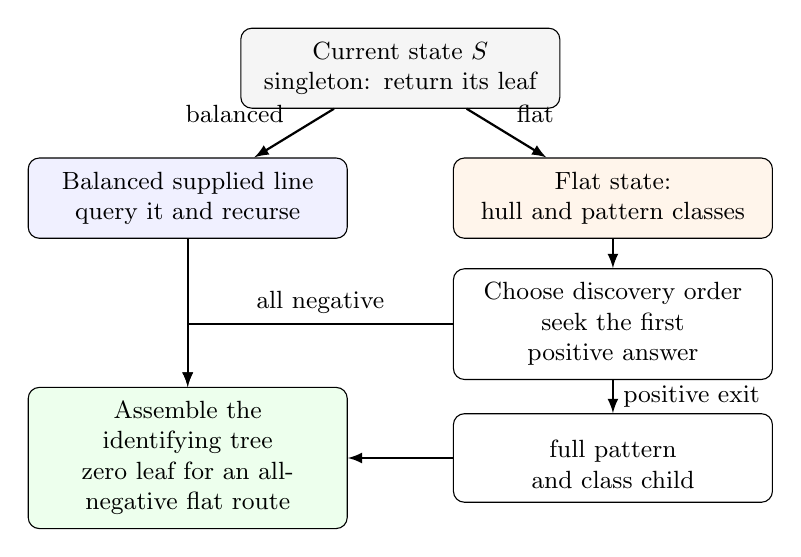
\begin{tikzpicture}[every node/.style={font=\small},
  box/.style={draw,rounded corners,align=center,inner sep=5pt,text width=3.7cm},
  arr/.style={-latex,thick}]
  \node[box,fill=gray!8] (state) at (0,0) {Current state $S$\\singleton: return its leaf};
  \node[box,fill=blue!6] (balanced) at (-2.7,-1.65)
    {Balanced supplied line\\query it and recurse};
  \node[box,fill=orange!8] (flat) at (2.7,-1.65)
    {Flat state: \HullData\\hull and pattern classes};
  \node[box] (discover) at (2.7,-3.25)
    {Choose discovery order\\seek the first positive answer};
  \node[box] (decode) at (2.7,-4.95)
    {\EndpointCode\\full pattern and class child};
  \node[box,fill=green!7] (output) at (-2.7,-4.95)
    {Assemble the identifying tree\\zero leaf for an all-negative flat route};
  \draw[arr] (state) -- node[above left]{balanced} (balanced);
  \draw[arr] (state) -- node[above right]{flat} (flat);
  \draw[arr] (flat) -- (discover);
  \draw[arr] (discover) -- node[right]{positive exit} (decode);
  \draw[arr] (discover.west) -- node[above]{all negative} (-2.7,-3.25)
    -- (output.north);
  \draw[arr] (decode) -- (output);
  \draw[arr] (balanced) -- (output);
\end{tikzpicture}
\caption{The common recursive structure. Arrows describe the output of
one stage passed to the next. The maximum-depth routines construct class
children before choosing the schedule, so their stored heights can set
deadlines; expected-depth routines use original prior masses. The flat
stage has an all-negative leaf only when the zero pattern is present.
Scheduling and decoding use supplied hull lines.}
\label{fig:recursive-procedure-flow}
\end{figure}



\subsection{Binary codes and ordered comparisons}

\begin{definition}[Binary codes and prefix codes]\label{def:binary-code}
A \emph{binary word} is a finite sequence of bits from $\{0,1\}$;
$\{0,1\}^*$ includes the empty word $\varepsilon$, of length zero.
A \emph{binary code} on a finite nonempty alphabet $\mathcal A$ is
an injective map $c:\mathcal A\to\{0,1\}^*$. The word $c(a)$ is
the \emph{codeword} for $a$, and $\ell_a=|c(a)|$ is its length.
A word $u$ is a \emph{prefix} of $v$ if $v$ starts with all the
bits of $u$. A code is \emph{prefix-free}, or a \emph{prefix code},
if no codeword is a prefix of another distinct codeword.
\end{definition}

For a distribution $(q_a)$ on the alphabet, the code's maximum
length is $\max_a\ell_a$ and its expected length is
$\sum_a q_a\ell_a$.
The prefix tree of a code has one node for each prefix of a
codeword, with the empty prefix at the root and edges appending
$0$ or $1$. For a prefix code its codewords are exactly the leaves,
at depths $\ell_a$. Conversely, the root-to-leaf answer words of
any binary decision tree form a prefix code. Unary nodes, which
have only one child, can be contracted without increasing any depth.
The empty word is permissible only when the alphabet is a singleton.
For example, $c(a)=0$, $c(b)=10$, and $c(c)=11$ form a prefix code
with lengths $1,2,2$.

\begin{definition}[Alphabetic codes]\label{def:alphabetic-code}
For an ordered alphabet $y_1<\cdots<y_r$, a prefix code is
\emph{alphabetic} if its codewords occur in that same lexicographic
order, with $0<1$. An \emph{ordered threshold comparison} asks
whether the unknown outcome is at most $y_j$ for some $j$.
\end{definition}

In an alphabetic prefix tree, the outcomes below each node form
a consecutive range. After unary nodes are contracted, its two
children separate that range at one threshold. Thus an alphabetic
code can be implemented by ordered threshold comparisons whenever
those comparisons are available. The code bits label the two
ordered ranges; a line's raw sign answer is routed to the matching
range, even if its sign encoding uses the opposite bit. This
relabeling adds no query. An arbitrary prefix code need
not be executable by the supplied line family. When we call an
identifying decision tree a \emph{code}, its internal queries must
still be supplied lines. Section~\ref{sec:endpoint-geometry} verifies
that the comparisons used for its endpoint codes are available.

A word $b_1\cdots b_\ell$ specifies the half-open \emph{dyadic cell}
\[
 D(b_1\cdots b_\ell)=
 \left[\sum_{j=1}^{\ell}b_j2^{-j},
       \sum_{j=1}^{\ell}b_j2^{-j}+2^{-\ell}\right)
 \subseteq[0,1).
\]
The empty word specifies $[0,1)$. Such cells are nested or disjoint;
one word is a prefix of another exactly when its cell contains
the other's cell. Half-open endpoints avoid ambiguity at dyadic
rationals.

\begin{theorem}[Kraft's inequality for binary prefix codes]
\label{thm:kraft}
Every finite binary prefix code has lengths satisfying
\[
 \sum_{a\in\mathcal A}2^{-\ell_a}\le1.
\]
Conversely, nonnegative integer lengths $(\ell_a)_{a\in\mathcal A}$
are realizable by a binary prefix code if this inequality holds.
The converse does not prescribe alphabetic order or guarantee
implementation by a restricted query family.
\end{theorem}
\begin{proof}
For necessity, prefix-free codewords specify disjoint dyadic cells
inside $[0,1)$, whose widths are $2^{-\ell_a}$.

For sufficiency, reorder the lengths as
$\ell_1\le\cdots\le\ell_r$ and put
$s_i=\sum_{j<i}2^{-\ell_j}$. Each $s_i$ is an integer multiple
of $2^{-\ell_i}$ because every earlier length is at most $\ell_i$.
The intervals $[s_i,s_i+2^{-\ell_i})$ are therefore dyadic cells
of the prescribed depths. They are disjoint and lie in $[0,1)$
by the assumed bound. Their binary descriptions give the required
prefix code; assign them back to the original symbols.
\end{proof}

The code $0,10,11$ has Kraft sum
$2^{-1}+2^{-2}+2^{-2}=1$. More generally, equality holds for a
proper binary tree because its two child cells partition each
internal node's cell. The coding facts here and the information
inequalities below are standard; see Cover and Thomas~\cite{ct2006}.

\subsection{Entropy and information inequalities}

\begin{definition}[Entropy and conditional entropy]\label{def:entropy}
A \emph{probability vector} $(q_i)$ has nonnegative entries summing
to one; its \emph{support} consists of the indices with $q_i>0$.
For a finite random variable $Y$ with probabilities
$q_y=\Pr[Y=y]$, its Shannon entropy in natural-log units is
\[
 H(Y)=-\sum_y q_y\ln q_y.
\]
We also write $H(q)$ for the entropy of a probability vector.
The joint entropy $H(Y,Z)$ is the entropy of the pair $(Y,Z)$.
For $Z$ with finite support, conditional entropy is
\[
 H(Y\mid Z)=
 \sum_{z:\Pr[Z=z]>0}\Pr[Z=z]\,H(Y\mid Z=z),
\]
where the inner entropy uses
$\Pr[Y=y\mid Z=z]=\Pr[Y=y,Z=z]/\Pr[Z=z]$.
Conditioning on several variables means
conditioning on their tuple. Entropy in bits is $H(Y)/\ln2$.
For a function $g$ of a finite random variable,
$\mathbb E[g(Y)]=\sum_y q_y g(y)$.
The \emph{binary entropy} is
$h(t)=-t\ln t-(1-t)\ln(1-t)$ for $0\le t\le1$.
\end{definition}

For nonempty $S$, the conditional hypothesis probabilities are
$q_h=\pi_h/w(S)$. Define the \emph{weighted state entropy} by
\[
 \mathcal E(S)=w(S)H(q)
       =\sum_{h\in S}\pi_h\ln\frac{w(S)}{\pi_h},
 \qquad \mathcal E(\varnothing)=0.
\]
It is zero on singletons. Like $c_{\mathrm E}$, this quantity
includes the original state mass rather than renormalizing it away.

\begin{lemma}[Log-sum inequality]\label{lem:log-sum}
For nonnegative $a_i$ and positive $b_i$, with
$A=\sum_i a_i>0$ and $B=\sum_i b_i$, one has
\[
 \sum_i a_i\ln\frac{a_i}{b_i}\ge A\ln\frac AB,
\]
with zero summands interpreted by continuity.
\end{lemma}
\begin{proof}
Put $q_i=a_i/A$ and $r_i=b_i/B$.
The inequality $-\ln x\ge1-x$ for $x>0$ follows because
$x-1-\ln x$ has its minimum zero at $x=1$. Hence
\[
 \sum_{i:q_i>0}q_i\ln\frac{q_i}{r_i}
 \ge\sum_{i:q_i>0}(q_i-r_i)
 =1-\sum_{i:q_i>0}r_i\ge0.
\]
Multiplying by $A$ and adding $A\ln(A/B)$ proves the assertion.
\end{proof}

\begin{lemma}[Entropy chain rule]\label{lem:entropy-chain-rule}
For finite random variables,
\[
 H(Y,Z)=H(Z)+H(Y\mid Z),\qquad
 H(Y,Z\mid W)=H(Y\mid W)+H(Z\mid Y,W).
\]
If $Z$ is determined by $Y$, then
$H(Y)=H(Z)+H(Y\mid Z)$. Also,
$0\le H(Y)\le\ln|\operatorname{supp}(Y)|$ and
$H(Y\mid Z)\ge0$; in particular $0\le h(t)\le\ln2$.
\end{lemma}
\begin{proof}
Substitute
$\Pr[Y=y,Z=z]=\Pr[Z=z]\Pr[Y=y\mid Z=z]$ into the joint
entropy sum. Taking its logarithm separates the two terms of the
first identity. Apply the same identity under each value of $W$
and average to obtain the conditional form. If $Z$ is determined
by $Y$, the pair $(Y,Z)$ has the same entropy as $Y$.
Entropy and conditional entropy are nonnegative because their
summands are $-q\ln q\ge0$ for $q\in[0,1]$.
Applying Lemma~\ref{lem:log-sum} to $Y$'s distribution and the
uniform distribution on its support gives the upper bound.
\end{proof}

\begin{lemma}[Alphabetic threshold codes]\label{lem:alphabetic-endpoints}
Let $Y$ have finite ordered support, and let $H(Y)$ be its entropy
with natural logarithms. There is an explicit alphabetic threshold
code with depth on outcome $y$ at most
$\log_2(1/\Pr[Y=y])+2$.
In particular its expected depth is at most
\[
 \frac{H(Y)}{\ln2}+2.
\]
This is a dyadic prefix-code construction; see Cover and
Thomas~\cite{ct2006} for the general coding background. The short
proof here also verifies the extra alphabetic (order-preserving)
property needed for threshold queries.
An optimal expected-depth threshold tree can also be computed by
a polynomial interval dynamic program. The explicit code is used
when the pointwise depth bound is needed.
\end{lemma}
\begin{proof}
For an ordered outcome $y$ of probability $a$, let
$F_y=\sum_{y'<y}\Pr[Y=y']$. Its \emph{cumulative-probability
interval} is $[F_y,F_y+a)$, with midpoint $m_y=F_y+a/2$.
The \emph{midpoint-dyadic code} chooses the dyadic cell containing
$m_y$ at depth $\ell_y=\lceil\log_2(2/a)\rceil$, in the sense
of the cells defined before Theorem~\ref{thm:kraft}.
The cell's width is at most $a/2$, so the entire cell lies in
the outcome's interval. These cells are disjoint and appear in
outcome order. Their binary descriptions form a prefix-free
alphabetic code. Since $\lceil x\rceil\le x+1$, their lengths
satisfy
\[
 \left\lceil\log_2\frac2a\right\rceil
 \le\log_2\frac1a+2.
\]
After unary nodes are contracted, each internal node separates
two consecutive outcome ranges and is a threshold comparison.
Taking expectation of this pointwise bound gives
\[
 \sum_y\Pr[Y=y]\left(\log_2\frac1{\Pr[Y=y]}+2\right)
 =\frac{H(Y)}{\ln2}+2.
\]

To minimize expected depth, let $D_{i,j}$ be the minimum weighted
depth contributed by outcomes $y_i,\ldots,y_j$, using their original
probabilities $p_a=\Pr[Y=y_a]$. Set $D_{i,i}=0$. For $i<j$, a root
threshold after $y_t$ contributes $\sum_{a=i}^j p_a$, so
\[
 D_{i,j}=\sum_{a=i}^j p_a+
       \min_{i\le t<j}\{D_{i,t}+D_{t+1,j}\}.
\]
This interval dynamic program uses $O(r^3)$ rational arithmetic
operations. The resulting optimal alphabetic tree satisfies the
expected-depth bound; no long binary expansion of a very small
probability is required. It need not preserve the pointwise bound,
which uses the explicit midpoint-dyadic construction.
\end{proof}

\begin{algorithm}[H]
\caption{Alphabetic code on ordered outcomes}
\label{alg:alphabetic-code}
\KwIn{Ordered outcomes $y_1<\cdots<y_r$ of positive rational masses $a_i$;
mode \emph{pointwise} or \emph{expected}.}
\KwOut{A threshold-comparison tree.}
\If{$r=1$}{\KwRet its zero-depth leaf\;}
\eIf{mode is \emph{pointwise}}{
  Normalize $q_i=a_i/\sum_j a_j$ and put $F_i=\sum_{j<i}q_j$\;
  \ForEach{$i$}{
    Find $d_i=\lceil\log_2(1/q_i)\rceil+1$ by rational powers-of-two comparisons\;
    Take the depth-$d_i$ dyadic cell containing $F_i+q_i/2$ as codeword $i$\;
  }
  Build the alphabetic prefix tree and contract unary nodes\;
}{
  Set $D_{i,i}=0$\;
  \For{$h=2,\ldots,r$}{
    \ForEach{$[i,j]$ of length $h$}{
      $D_{i,j}\gets\sum_{a=i}^j a_a+min_{i\le t<j}(D_{i,t}+D_{t+1,j})$\;
      Store a minimizing split after $y_t$\;
    }
  }
  Reconstruct the stored interval splits\;
}
\KwRet the ordered tree, implementing each split by its available threshold\;
\end{algorithm}

The pointwise mode preserves the per-outcome bound; the expected mode
has $O(r^3)$ arithmetic complexity and avoids long expansions for small
priors. Their distinct roles are proved in
Lemma~\ref{lem:alphabetic-endpoints}.


\subsection{Restriction and recursive accounting}

Two lower bounds will account for different kinds of work.
Restriction measures which queries are unnecessary once a class
is known. Entropy measures the information learned from a class label.

\begin{definition}[Partitions and refinement]\label{def:partitions}
A \emph{partition} $\Pi$ of $S$ is a family of pairwise disjoint
nonempty subsets whose union is $S$. We say $\Pi$ \emph{refines}
$\mathcal R$, or $\mathcal R$ is \emph{coarser} than $\Pi$, if
every class of $\Pi$ is contained in a class of $\mathcal R$.
The output classes of a partial decision tree form a partition.
\end{definition}

\begin{lemma}\label{lem:restriction}
For pairwise disjoint subsets $S_1,\ldots,S_k$ of a state $S$,
\[
 \sum_i \OPT_{\mathrm E}(S_i)\le \OPT_{\mathrm E}(S),\qquad
 \OPT_{\mathrm W}(S_i)\le \OPT_{\mathrm W}(S).
\]
Moreover,
\[
 \OPT_{\mathrm E}(S)\ge\frac{\mathcal E(S)}{\ln2},
 \qquad
 \OPT_{\mathrm W}(S)\ge\frac{\ln|S|}{\ln2}
 \quad\text{for nonempty }S.
\]
\end{lemma}
\begin{proof}
Restrict an optimal tree on $S$ to each $S_i$ and contract its constant
queries. No hypothesis's depth increases. Summing over disjoint
subsets proves the expected-depth inequality; restricting a
maximum-depth-optimal tree proves the second inequality.

For entropy, assume $S\ne\varnothing$; the empty-state case is
immediate. Let $q_h=\pi_h/w(S)$. The leaf transcripts are a binary
prefix code as in Definition~\ref{def:binary-code}: a transcript
cannot continue beyond a leaf. Theorem~\ref{thm:kraft} therefore
gives $\sum_h2^{-\ell_h}\le1$ for their lengths.
Apply Lemma~\ref{lem:log-sum}, dividing by $\ln2$ to use base two, with
$\ell_h=d_T(h)$ and $q_h=\pi_h/w(S)$:
\[
 \begin{aligned}
 \sum_h q_h\ell_h-\sum_hq_h\log_2\frac1{q_h}
 &=\sum_hq_h\log_2\frac{q_h}{2^{-\ell_h}}\\
 &\ge \log_2\frac{\sum_hq_h}{\sum_h2^{-\ell_h}}
 \ge0.
 \end{aligned}
\]
The first inequality is the log-sum inequality, and the second uses
$\sum_hq_h=1$ and Kraft's bound. Hence every tree identifying $S$
satisfies
\[
 c_{\mathrm E}(T)=w(S)\sum_hq_hd_T(h)
 \ge w(S)\sum_hq_h\log_2\frac1{q_h}
 =\frac{w(S)}{\ln2}\sum_hq_h\ln\frac1{q_h}
 =\frac{\mathcal E(S)}{\ln2}.
\]
Minimizing gives the expected-depth lower bound.
For the maximum-depth bound, prove by induction on $d$ that a binary
tree of height $d$ has at most $2^d$ leaves. The claim is immediate
for $d=0$; for $d>0$, the root has at most two child subtrees, each
of height at most $d-1$, so together they have at most
$2\cdot2^{d-1}=2^d$ leaves. Thus $|S|\le2^d$, or
$d\ge\log_2|S|=\ln|S|/\ln2$.
\end{proof}

We call a state quantity used to account for progress a
\emph{potential}. For expected depth, the relevant potentials
are $\OPT_{\mathrm E}$ and $\mathcal E$; their decrements are the
parent value minus the sum of the child values.
For a nonempty state $S$ and a partition $\Pi$ of it, write
\[
 \begin{split}
  \Delta_{\mathrm E}(S,\Pi)&=\OPT_{\mathrm E}(S)
                     -\sum_{A\in\Pi}\OPT_{\mathrm E}(A),\\
  I(S,\Pi)&=\mathcal E(S)-\sum_{A\in\Pi}\mathcal E(A)
           =\sum_{A\in\Pi}w(A)\ln\frac{w(S)}{w(A)}.
  \end{split}
 \]
  Let $X$ be a random hypothesis with
 $\Pr[X=h]=\pi_h/w(S)$, and let $P$ be its class label under $\Pi$.
 Then
 \[
  I(S,\Pi)=w(S)H(P),\qquad
  H(P)=-\sum_{A\in\Pi}\frac{w(A)}{w(S)}
                          \ln\frac{w(A)}{w(S)}.
 \]
 Thus $I(S,\Pi)$ is the state mass times the Shannon entropy of the
 class label, measured in natural-log units. This is the partition
 form of the chain rule in Lemma~\ref{lem:entropy-chain-rule}.
 Both quantities are nonnegative. The first is the decrease in
optimal expected depth when the class is revealed; the second is
the weighted entropy of that class. Their differences telescope
over any recursive partition ending in singletons. More explicitly,
if each internal state $S$ is split into classes $\Pi_S$, then
\[
 \sum_{S\ {\rm internal}}\Delta_{\mathrm E}(S,\Pi_S)
       =\OPT_{\mathrm E}(\HH),\qquad
 \sum_{S\ {\rm internal}}I(S,\Pi_S)=\mathcal E(\HH).
\]
Every child term cancels against that child's term at its own split,
and the terminal singleton potentials are zero. The approximation
proofs will bound each stage by these local decreases; this
cancellation is what prevents repeated charges to the same optimum.

\subsection{Convex geometry and finite set systems}

\begin{definition}[Planar convexity]\label{def:convex-geometry}
A set is \emph{convex} if it contains the segment joining any two
of its points. A \emph{convex combination} is a sum
$\sum_j\lambda_j u_j$ with $\lambda_j\ge0$ and
$\sum_j\lambda_j=1$. The \emph{convex hull}
$\operatorname{conv}(U)$ of a finite nonempty point set $U$ is the set of
its convex combinations. A \emph{vertex}, or extreme point, cannot
be expressed as a convex combination of other points of the hull.
The hull is the convex hull of its vertices; set
$\operatorname{conv}(\varnothing)=\varnothing$ by convention.

A nonempty planar hull has affine dimension zero, one, or two according
as it is a point, a nontrivial segment, or has nonempty planar
interior. In dimension two it is a convex polygon, whose vertices
have a cyclic boundary order; its \emph{edges} join consecutive
vertices. A \emph{supporting line} meets a convex set and leaves
it entirely on one closed side. It \emph{exposes} a point if that
point is its unique intersection with the set. A finite point
set is in \emph{strictly convex position} if every point is a
vertex of its hull.
\end{definition}

An open half-plane has the form $\{x:a\cdot x>b\}$ for $a\ne0$;
replacing $>$ by $\ge$ gives its closed counterpart. A point is
\emph{strictly} on a chosen side when it is in that open half-plane,
not on its boundary. A common strict \emph{witness} for several
chosen sides is a point in all their open half-planes; it need
not itself be a hypothesis.

\begin{theorem}[Planar Helly theorem]\label{thm:helly}
If every subfamily of at most three
sets in a finite family of planar convex sets has nonempty
intersection, then the whole family has nonempty intersection.
The sets may be open.
\end{theorem}
This is the standard planar form; see Matou\v{s}ek~\cite{matousek2002}.

\begin{definition}[Covers and hitting sets]\label{def:covers-and-hitting}
A finite \emph{set system} consists of a universe $U$, a candidate
set $V$, and supplied subsets $F_v\subseteq U$ indexed by $v\in V$.
A \emph{cover} of $U$ is a choice of these sets whose union contains
every element of $U$.
In the equivalent demand formulation, there is a candidate set $V$
and a subset $D_h\subseteq V$ for each demand $h$. A \emph{hitting
set} is a subset $P\subseteq V$ with $P\cap D_h\ne\varnothing$
for every demand. Choosing $v$ covers exactly
$F_v=\{h:v\in D_h\}$. Thus covering demands by candidates and
hitting their subsets are the same incidence problem.
A demand with $D_h=\varnothing$ is uncoverable.
\end{definition}

With positive demand weights, the weight covered by a choice is
the sum of weights of demands hit at least once; repeated hits
are not counted again. An \emph{incidence table} records the bits
$\mathbf1[h\in F_v]$, equivalently $\mathbf1[v\in D_h]$.
A cardinality budget is a nonnegative integer $k$ permitting at
most $k$ selected candidates. We may cap it at $|V|$, since there
are no more distinct candidates to choose.

\begin{definition}[Ordered and circular intervals]\label{def:ordered-intervals}
On a finite linear order $v_1,\ldots,v_M$, an \emph{ordinary
interval} is a consecutive subset $\{v_i,\ldots,v_j\}$; we also
allow the empty interval. Its nonempty intervals have first and
last elements, called their endpoints.
On a cyclic order, a \emph{circular interval} is a consecutive
block with wrap-around allowed, also permitting the empty and
whole-cycle sets. Two vertices are \emph{adjacent} when consecutive
in this order, including $v_M,v_1$ on a cycle. An \emph{oriented
adjacent pair} specifies which of those two vertices is first.
A \emph{run} of $P$ in a linear candidate order is a maximal
nonempty consecutive block contained in $P$; $c(P)$ counts such
runs, with $c(\varnothing)=0$.
\end{definition}

Cutting a cyclic order at a removed vertex turns any circular
interval avoiding that vertex into an ordinary interval.
When interval demands occur below, candidates are the ordered
vertices, and a demand is hit by selecting a vertex in its interval,
not by selecting the interval itself.

\subsection{Query orderings and first-cover costs}

Let a universe $U$ have positive element weights $\pi_h$ and supplied
sets $F_v$ covering $U$. These weights need not sum to one.
A \emph{cover ordering}
$Q=(F_{v_1},\ldots,F_{v_\ell})$ is a sequence of distinct supplied
sets whose union covers $U$, and $|Q|=\ell$ is its length.
The \emph{first-cover time}, or \emph{latency}, of $h$ is
$t_Q(h)=\min\{j:h\in F_{v_j}\}$.
The \emph{weighted min-sum set cover} objective is
\[
 \MSSC(Q)=\sum_{h\in U}\pi_h t_Q(h).
\]
Equivalently, $\MSSC(Q)$ is the sum of the uncovered mass before
each step:
\[
 \MSSC(Q)=
 \sum_{j=0}^{|Q|-1}
 w\left(U\setminus\bigcup_{r=1}^{j}F_{v_r}\right),
 \qquad w(E)=\sum_{h\in E}\pi_h.
\]
The union for $j=0$ is empty. \emph{Maximum-remaining-weight greedy}
repeatedly chooses the supplied set containing the largest total
weight of elements not yet covered, counting each element only once.

\subsection{Normalized queries and hull patterns}

\begin{definition}[Witness-relative query notation]\label{def:normalized-queries}
Enumerate the supplied lines as $\ell_1,\ldots,\ell_m$.
For a state $S$ and a point $p$ on no supplied line, put
\[
 x_h=h-p,\qquad
 u_i=-\frac{a_{\ell_i}}{f_{\ell_i}(p)},\qquad
 C_i=\{y:u_i\cdot(y-p)>1\}.
\]
Thus $x_h$ is a translated hypothesis vector, $u_i$ a normalized
query vector, and $C_i$ the cap opposite $p$ in the original plane.
The corresponding dual demand is
\[
 R_h=\{u:u\cdot x_h>1\}.
\]
Write $K=\operatorname{conv}(\{0\}\cup\{u_i:i\in[m]\})$ and let
$V$ be its nonzero vertices, in cyclic hull order.
Every $v\in V$ equals a supplied query vector; choose one
representative line if several coincide, and put
$C_v=\{y:v\cdot(y-p)>1\}$.
A \emph{support block} $J_i\subseteq V$ represents $u_i$ as
$u_i=\sum_{v\in J_i}\alpha_{iv}v$, with positive coefficients
and $\sum_v\alpha_{iv}\le1$. We choose blocks of at most two
vertices, adjacent when there are two; their existence is proved
in Lemma~\ref{lem:hull-structure}.
\end{definition}

The origin is a known-negative marker, not a query, since
$0\cdot x_h=0$. If it lies on the hull boundary, it can be inserted
at its boundary position as a free cut marker. The hull $K$, its
vertices, and their cyclic order can be computed in polynomial time
by standard planar convex-hull algorithms~\cite{deberg2008}.

Indeed,
\[
 u_i\cdot x_h-1=-\frac{f_{\ell_i}(h)}{f_{\ell_i}(p)}.
\]
Consequently, $h\in C_i$ exactly when $u_i\in R_h$, and equality
$u_i\cdot x_h=1$ means $h$ lies on $\ell_i$.
We encode the cap-side answer as $1$ and the witness-side answer
as $0$. A \emph{positive hull answer} is this cap-side bit,
regardless of the original affine sign. This relabeling introduces
no new query. If $x_h=0$, the demand $R_h$ is empty.
Intersections such as $C_i\cap S$ always contain the original
hypotheses $h$, not their translated vectors.

\begin{definition}[Hull patterns and pattern classes]\label{def:hull-pattern}
The \emph{hull pattern} of $h\in S$ is the bit vector
\[
 \sigma(h)=\bigl(\mathbf1[v\cdot x_h>1]\bigr)_{v\in V}.
\]
A \emph{pattern class} consists of all hypotheses with the same
vector, and $\Pi$ is the partition into these classes.
The \emph{positive vertices} are the coordinates whose bits are one.
Write $A_0$ for the class with every bit zero, taking
$A_0=\varnothing$ when no hypothesis has that pattern.
When a prior is specified, the nonzero-pattern mass is
$b(S)=w(S)-w(A_0)$, the mass on which a positive hull answer is possible.
\end{definition}

A \emph{discovery schedule} lists individual hull tests in their
query order along the all-negative route. Its \emph{first-hit time}
$g_A$ for a nonzero pattern class is the index of the first listed
vertex positive on that class.
